\section{Lab1b - Netzwerkanalyse}

\subsection{Direkt erreichbare Netze}

Im ersten Schritt war zu ermitteln, welche Netzwerke vom Tomcat-Server aus direkt zu erreichen sind. Die Antwort darauf liefert das Auslesen der sogenannten Kernel Routing Tables mit Hilfe von netstat.

\begin{lstlisting}
walter@tomcat:~$ netstat -rn
Kernel IP routing table
Destination     Gateway         Genmask         Flags   MSS Window  irtt Iface
192.168.20.0    0.0.0.0         255.255.255.0   U         0 0          0 eth0
192.168.98.0    0.0.0.0         255.255.255.0   U         0 0          0 eth1.98
0.0.0.0         192.168.98.1    0.0.0.0         UG        0 0          0 eth1.98
walter@tomcat:~$ netstat -6rn
Kernel IPv6 routing table
Destination                    Next Hop                   Flag Met Ref Use If
fdcb:c447:e9d2:3553:1001::/120 ::                         U    256 0
  1 eth1.98
fe80::/64                      ::                         U    256 0     0 eth0
fe80::/64                      ::                         U    256 0     0 eth1
fe80::/64                      ::                         U    256 0
  0 eth1.98
::/0                           fdcb:c447:e9d2:3553:1001::1 UG   1024
1224143 eth1.98
::/0                           ::                         !n   -1  1246254 lo
::1/128                        ::                         Un   0   3    28 lo
fdcb:c447:e9d2:3553:1001::ab/128 ::                         Un   0   1 76668 lo
fe80::21b:d7ff:fe12:bc52/128   ::                         Un   0   1  2235 lo
ff00::/8                       ::                         U    256 0     0 eth0
ff00::/8                       ::                         U    256 0     0 eth1
ff00::/8                       ::                         U    256 0
  0 eth1.98
::/0                           ::                         !n   -1  1246254 lo
\end{lstlisting}

Die direkt erreichbaren Netze sind daher: 192.168.20.0/24 und 192.168.98.0/24

\subsection{Ping-Scan}

Im nächsten Schritt war ein Ping-Scans durchzuführen, um zu ermitteln, welche Hosts in den genannten IP-Adress-Bereichen erreichbar sind. Die zu durchsuchenden Bereich waren dabei: 192.168.96.0/21, 172.16.0.0/22, 10.12.0.0/24 für IPv4 sowie fdcb:c447:e9d2:3553:1000::/120 bis fdcb:c447:e9d2:3553:100f::/120.

Die Scans der IPv4-Adresse konnten wir direkt auf dem Server durchführen:

\begin{lstlisting}
walter@tomcat:~$ nmap -v -sP 192.168.96.0/21 | grep up
Host omega.local.vienna.essecorp.invalid (192.168.98.1) is up (0.0023s latency).
Host alpha.local.vienna.essecorp.invalid (192.168.98.10) is up (0.00054s latency).
Host beta.local.vienna.essecorp.invalid (192.168.98.28) is up (0.00023s latency).
Host gamma.local.vienna.essecorp.invalid (192.168.98.54) is up (0.00035s latency).
Host delta.local.vienna.essecorp.invalid (192.168.98.99) is up (0.0031s latency).
Host tomcat.local.vienna.essecorp.invalid (192.168.98.124) is up (0.000076s latency).
Host epsilon.local.vienna.essecorp.invalid (192.168.98.201) is up (0.00038s latency).
Host zeta.local.vienna.essecorp.invalid (192.168.98.202) is up (0.0015s latency).
Nmap done: 2048 IP addresses (8 hosts up) scanned in 87.47 seconds

walter@tomcat:~$ nmap -v -sP 172.16.0.0/22 | grep up
Host gemini.dmz.vienna.essecorp.invalid (172.16.2.12) is up (0.0065s latency).
Host phoenix.dmz.vienna.essecorp.invalid (172.16.2.15) is up (0.0035s latency).
Host taurus.dmz.vienna.essecorp.invalid (172.16.2.25) is up (0.0041s latency).
Host lyra.dmz.vienna.essecorp.invalid (172.16.2.253) is up (0.00070s latency).
Nmap done: 1024 IP addresses (4 hosts up) scanned in 78.61 seconds

walter@tomcat:~$ nmap -v -sP 10.12.0.0/24 | grep up
Nmap done: 256 IP addresses (0 hosts up) scanned in 104.14 seconds
\end{lstlisting}

Da nmap beim Scan von IPv6-Adressen keine Adressebereiche unterstütz, mussten wir uns für diesen Teil der Aufgabe ein kleines Python-Skript schreiben, das die gewünschten Adressen erzeugt und dann für jede einzelne Adresse nmap aufruft.
Eine weitere Komplikation ergab sich, da wir auf dem Tomcat-Server keinerlei Schreibrechte hatten. Aus diesem Grund konnten wir weder das Skript selbst auf dem Server ablegen, noch den Output des Skripts in eine Datei auf dem Server schreiben, um sie später zur Analyse zur Verfügung zu haben. Um dies zu umgehen, ließen wir das Skript auf einem unserer Rechner lokal laufen und riefen im Skript nmap über ssh auf dem Server auf:

\begin{lstlisting}
import subprocess

for y in range (0, 16):
  base_address = "fdcb:c447:e9d2:3553:100" + format(y, 'x') + ":0000:0000:00"
  for x in range (0, 256):
    address = base_address + format(x, 'x')
    subprocess.call(['ssh', '-p 2222', 'walter@localhost', 'nmap', '-6', '-sP', address])
\end{lstlisting}

Der Aufruf des Skripts bringt folgendes Ergebnis:

\begin{lstlisting}
david@brazos:~/lab1$ python ipv6-scan.py > output.txt
david@brazos:~/lab1$ cat output.txt | grep fdcb
Host omega.local.vienna.essecorp.invalid (fdcb:c447:e9d2:3553:1001::1) is up (0.0041s latency).
Host alpha.local.vienna.essecorp.invalid (fdcb:c447:e9d2:3553:1001::5) is up (0.0044s latency).
Host beta.local.vienna.essecorp.invalid (fdcb:c447:e9d2:3553:1001::9) is up (0.0041s latency).
Host gamma.local.vienna.essecorp.invalid (fdcb:c447:e9d2:3553:1001::21) is up (0.0027s latency).
Host delta.local.vienna.essecorp.invalid (fdcb:c447:e9d2:3553:1001::43) is up (0.0064s latency).
Host epsilon.local.vienna.essecorp.invalid (fdcb:c447:e9d2:3553:1001::79) is up (0.0064s latency).
Host zeta.local.vienna.essecorp.invalid (fdcb:c447:e9d2:3553:1001::88) is up (0.0064s latency).
Host tomcat.local.vienna.essecorp.invalid (fdcb:c447:e9d2:3553:1001::ab) is up (0.000044s latency).
Host lyra.dmz.vienna.essecorp.invalid (fdcb:c447:e9d2:3553:1002::fd) is up (0.00021s latency).
Host kerberos.dmz.vienna.essecorp.invalid (fdcb:c447:e9d2:3553:1002::fe) is up (0.00049s latency).
Host athena.extra.atlanta.essecorp.invalid (fdcb:c447:e9d2:3553:1003::7f) is up (0.26s latency).
Host zeus.extra.atlanta.essecorp.invalid (fdcb:c447:e9d2:3553:1003::9a) is up (0.27s latency).
Host kerberos.extra.atlanta.essecorp.invalid (fdcb:c447:e9d2:3553:1003::da) is up (0.00046s latency).
\end{lstlisting}

\subsection{Port-Scans}
Als nächstes scannten wir alle gefundenen Hosts auf offene Ports und laufende Services.
Nachfolgend werden die gefundenen IP-Adressen und ihre zugehörigen offenen Ports sowie Services aufgelistet:
TCP IPv4 Scans:
\begin{lstlisting}
192.168.98.10 Port 53 domain dnsmasq 2.55
192.168.98.28 Port 25 SMTP
192.168.98.54 Port 1080 socks5 (Username/password authentication required)
192.168.98.99 Port 631 ipp cups 1.4 (Printserver Apple)
192.168.98.124 Port 8000 Apache Tomcat/Coyote JSP engine 1.1
192.168.98.124 Port 8009 ajp13 Apache Server, Service Info: OS: Linux 
192.168.98.124 Port 22 OpenSSH 5.5p1 Debian 6+sqeueeze3 (Protocol 2.0), OS: Linux
192.168.98.201 Port 139 und 445 (Printserver smb mit und ohne netbios) netbios-ssn Samba smbd 3.X (workgroup: ESSECORP)
172.16.2.12 http lighttpd 1.4.28 dmz
172.16.2.15 Port 21 FTP vsftpd 2.3.2 dmz
172.16.2.25 Port 25 SMTP dmz
\end{lstlisting}

IPv6 Scans:
\begin{lstlisting}
athena.extra.atlanta.essecorp.invalid:
Port 80 - http ligthttpd
Port 443 - ssl/http lighttpd

zeus.extra.atlanta.essecorp.invalid:
Port 7 - echo
Port 9 - discard?
Port 13 - daytime
Port 19 - chargen Linux
Port 22 - ssh
Port 37 - time?
\end{lstlisting}

Der Netzwerkplan zeigt wie das Netzwerk aufgebaut ist.

\begin{figure}[h!]
  \centering
  \fbox{
    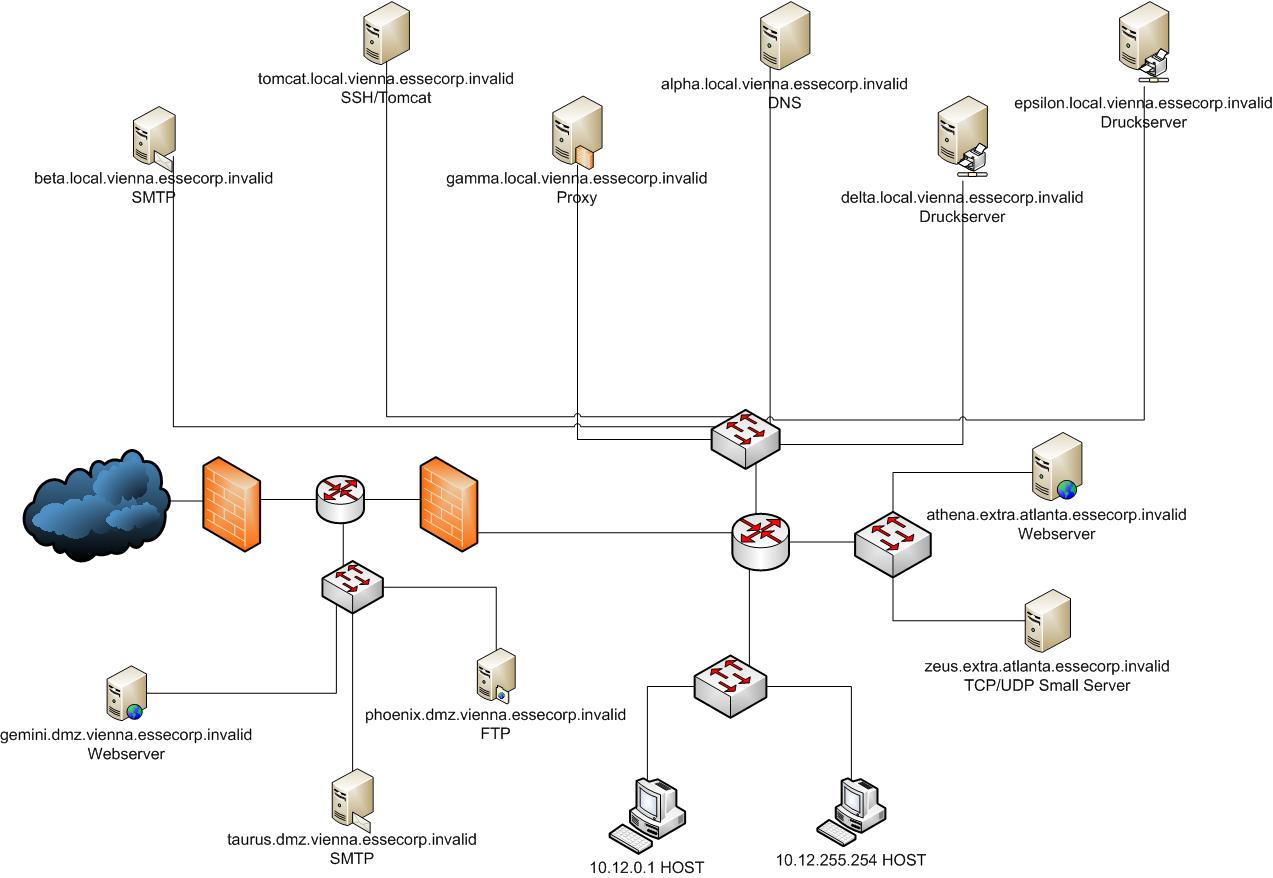
\includegraphics[width=1\textwidth]{./imgs/Netzwerkplan.jpg}
  }
  \caption{Netzwerkplan}
  \label{fig:netzwerkplan}
\end{figure}

Es fällt sofort auf, dass es 4 verschiedene große Domänen gibt, die jeweils eine andere Funktionalität verfolgen:
\begin{enumerate}
\item local.vienna.essegroup.invalid
\item dmz.vienna.essegroup.invalid
\item extra.atlanta.essegroup.invalid
\item Hosts
\end{enumerate}

Die erste lokale Domäne beinhaltet einen typischen Proxy, der innerhalb des lokalen Netzwerkes arbeitet. Außerdem gibt es einen
internen Mail-Server (SMTP), einen internen Tomcat mit SSH-Zugang, sowie den typischen DNS und 2 Druckerserver, die
nur intern genutzt werden können.\linebreak
Die DMZ (Demilitarisierte Zone) bietet Services an, auf die man auch aus dem Internet zugreifen kann. Somit existieren die
3 Komponenten Mailserver, FTP- und SMTP-Server.\linebreak
Die Komponenten TCP/UDP-Server, sowie ein kleiner Lightweight-HTTP-Webserver liegen hier in einer eigenen Domäne.\linebreak
Die Host bekommen Adressen im Bereich von 10.12.0.1 bis 10.12.255.254.
